\section{Zusammenstellung Signalformen}
\begin{table}[htdp]
\begin{center}
\begin{tabular}{|c|c|c|c|c|}
\hline
\textbf{Signal} & \textbf{Funktion} & \textbf{$X_0$} & \textbf{$X^2$} & \textbf{var(X)} \\

\hline
\parbox[c][2.1cm]{3.5cm}{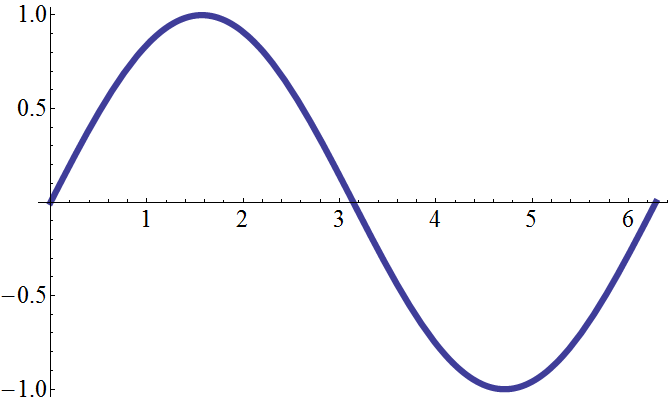
\includegraphics[height=2cm]{./bilder/Signale/Sinus.png}} &
$A\cdot\sin(t)$  & $0$ &
$\frac{A^2}{2}$ & $\frac{A^2}{2}$ \\

\hline
\parbox[c][2.1cm]{3.5cm}{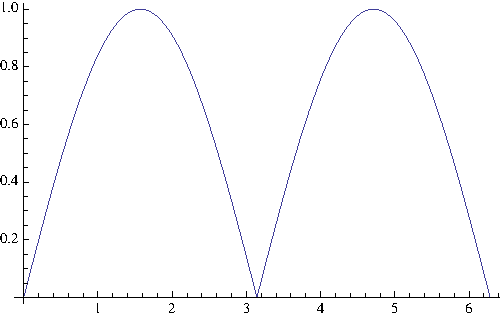
\includegraphics[height=2cm]{./bilder/Signale/absSinus.png}} &
$A\cdot|\sin(t)|$  &
$\frac{2A}{\pi}$ & $\frac{A^2}{2}$ & $\frac{A^2}{2}-\frac{4A^2}{\pi^2}$\\

\hline
\parbox[c][2.1cm]{3.5cm}{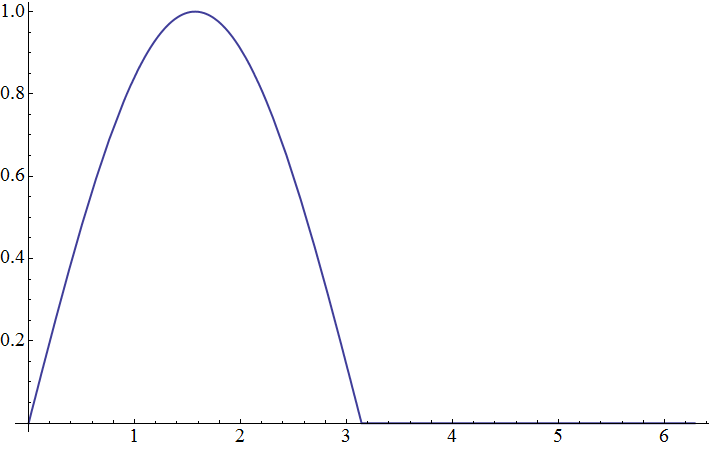
\includegraphics[height=2cm]{./bilder/Signale/Sinus_ersteWelle.png}} &
$\begin{cases} A\cdot\sin (t) & 0<t<\pi  \\ 0 & \text{True}\end{cases}$ & $\frac{A}{\pi}$ &
$\frac{A^2}{4}$ & $\frac{A^2}{4}-\frac{A^2}{\pi^2}$\\

\hline
\parbox[c][2.1cm]{3.5cm}{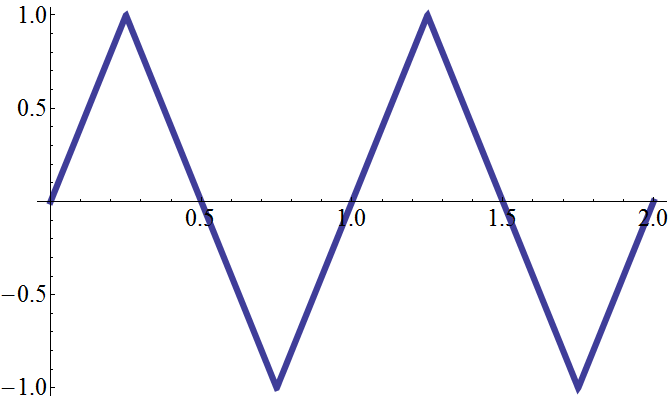
\includegraphics[height=2cm]{./bilder/Signale/Dreieck2.png}} &
$A\cdot\Lambda(t)$
& $0$ & $\frac{A^2}{3}$ &
$\frac{A^2}{3}$ \\

\hline
\parbox[c][2.1cm]{3.5cm}{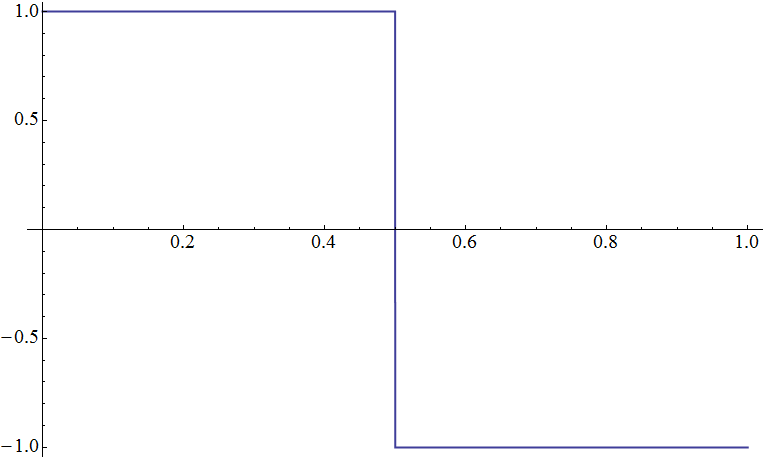
\includegraphics[height=2cm]{./bilder/Signale/UnitStep.png}} &
$A\cdot\prod(t)$
& $0$ & $A^2$ & $A^2$ \\

\hline
\parbox[c][2.1cm]{3.5cm}{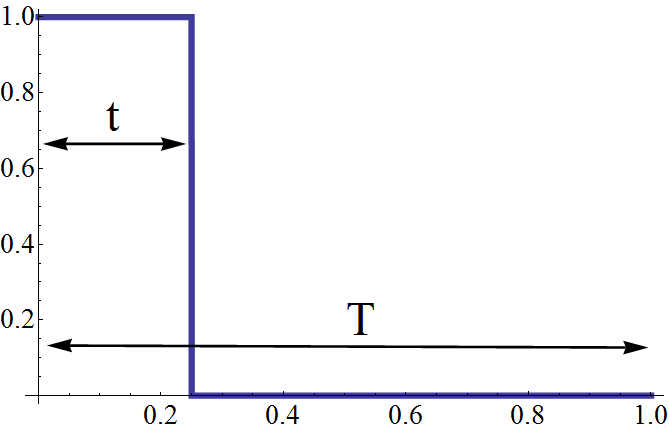
\includegraphics[height=2cm]{./bilder/Signale/StepAt_t.png}} &
$\begin{cases} A & 0<x<t \\ 0 & \text{True}\end{cases}$ 
& $A\frac{t}{T}$ &
$A^2\frac{t}{T}$ & $\frac{A^2t}{T}-\frac{A^2t^2}{T^2}$ \\

\hline
\end{tabular}
\end{center}
\end{table}